\section{Implementation}
In this section, we will describe the implementation of the timed automaton model from the previous section, shown in Figure \ref{fig:automaton}. Our tool of choice is UPPAAL, an integrated solution for modeling, simulation, and verification of timed automata. We will present the implementation of limitations imposed on the model in the following subsection.  Model variables representing its state will be described along with the most important functions.


\subsection{Model}
Implementation of the timed automaton, shown in Figure \ref{fig:implementation}, has an additional state called \texttt{grid} and global functions that abstract away the underneath complexity. This state is a consequence of imposing limitations on the environment size defined in the previous section. This allows us to reduce the state space size and perform verification. It is the biggest change made to the original algorithm, defined in Figure \ref{fig:pseudocode}. In that state, it is determined whether a robot has reached the boundary of the grid. If yes, the robot will transition to the state \texttt{turn\_180} and change its direction by 180 degrees as it cannot continue moving forward outside of its environment. If a robot has not reached the boundary of its environment it will transition to the \texttt{if} state where it will follow the original rules of the algorithm.

\begin{figure}[H]
\caption{UPPAAL implementation of the timed automaton}
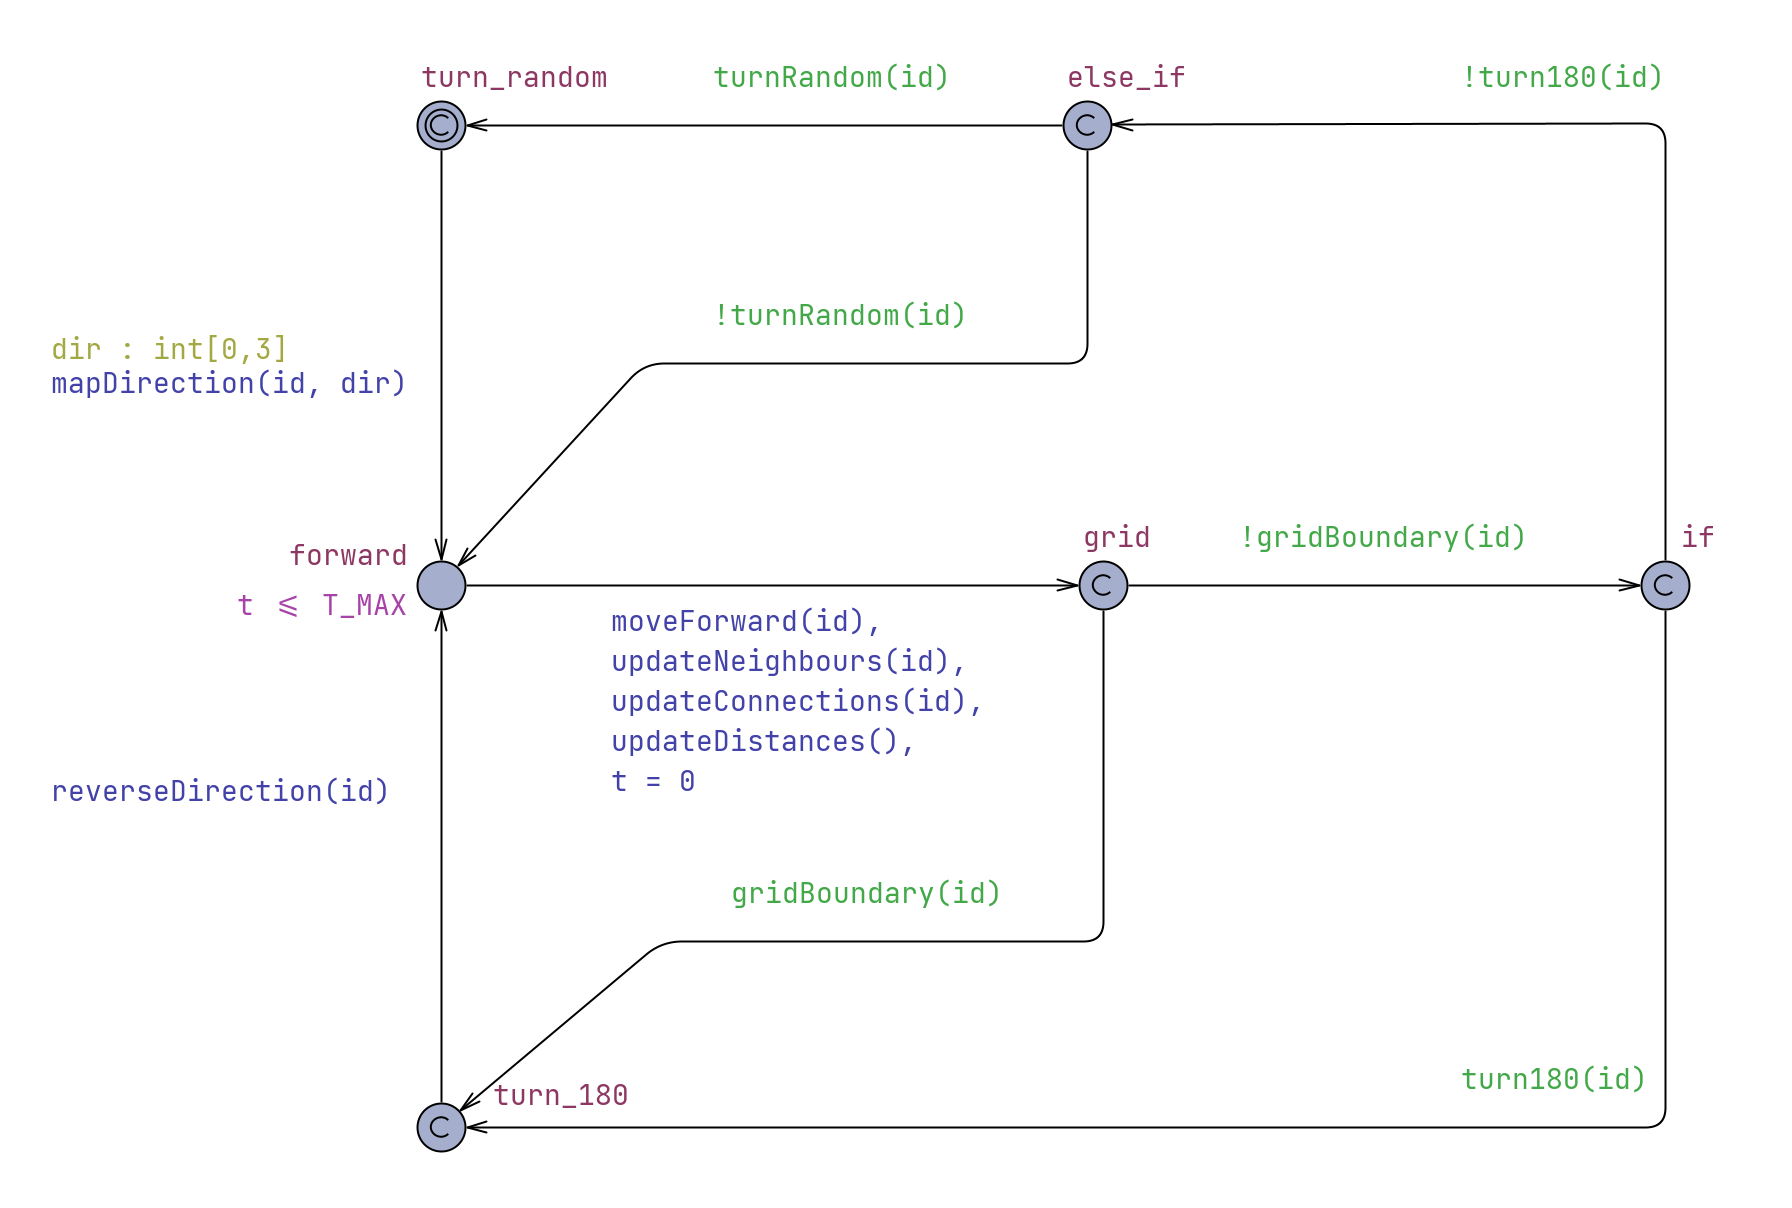
\includegraphics[width=\textwidth]{images/implementation.png}
\label{fig:implementation}
\end{figure}



\subsection{Movement}



\subsection{Connection}



\subsection{System variables}
